\documentclass[12pt,a4paper]{article}

% ─── Page Layout ───────────────────────────────────────────────────────────────
\usepackage[a4paper, margin=0.8in, headheight=14pt]{geometry}

% ─── Fonts (XeLaTeX) ───────────────────────────────────────────────────────────
\usepackage{fontspec}
\usepackage{unicode-math}
\setmainfont{TeX Gyre Pagella}
\setmonofont[Scale=0.88]{TeX Gyre Cursor}
\setmathfont{Latin Modern Math}

% ─── Packages ──────────────────────────────────────────────────────────────────
\usepackage{xcolor}
\usepackage{colortbl}
\usepackage{titlesec}
\usepackage{enumitem}
\usepackage{tabularx}
\usepackage{longtable}
\usepackage{booktabs}
\usepackage{array}
\usepackage{amsmath}
\usepackage{tikz}
\usetikzlibrary{shapes.geometric, arrows.meta, positioning, calc, fit, decorations.pathreplacing, patterns}
\usepackage{tcolorbox}
\tcbuselibrary{skins, breakable}
\usepackage{hyperref}
\usepackage{fancyhdr}
\usepackage{graphicx}
\usepackage{microtype}
\hyphenpenalty=10000
\exhyphenpenalty=10000
\sloppy
\usepackage{caption}
\usepackage{setspace}
\usepackage{multirow}
\usepackage{tocloft}

% ─── Q&A helper ────────────────────────────────────────────────────────────────
\newcommand{\Q}[1]{\textbf{#1}\par\noindent\ignorespaces}

% ─── Colour Palette ────────────────────────────────────────────────────────────
\definecolor{myred}{RGB}{196,30,58}
\definecolor{mydark}{RGB}{30,30,50}
\definecolor{mygreen}{RGB}{14,120,80}
\definecolor{myteal}{RGB}{0,130,140}
\definecolor{myamber}{RGB}{180,100,0}
\definecolor{mypurple}{RGB}{100,30,160}
\definecolor{mygray}{RGB}{246,247,249}
\definecolor{mgframe}{RGB}{180,185,200}
\definecolor{watermark}{RGB}{145,150,170}
\definecolor{hdrred}{RGB}{250,232,235}
\definecolor{hdrgreen}{RGB}{220,244,233}
\definecolor{hdrteal}{RGB}{220,242,244}
\definecolor{hdramber}{RGB}{253,242,215}
\definecolor{hdrpurple}{RGB}{238,228,255}
\definecolor{hdrgray}{RGB}{238,240,245}

% ─── Section Formatting ────────────────────────────────────────────────────────
\titleformat{\section}
  {\large\bfseries\color{myred}}{\thesection.}{0.5em}{}
  [\vspace{1pt}{\color{myred}\rule{\linewidth}{0.8pt}}]
\titleformat{\subsection}
  {\normalsize\bfseries\color{myteal}}{\thesubsection}{0.5em}{}
\titlespacing*{\section}{0pt}{18pt}{7pt}
\titlespacing*{\subsection}{0pt}{11pt}{4pt}

% ─── Paragraph ─────────────────────────────────────────────────────────────────
\setlength{\parindent}{0pt}
\setlength{\parskip}{4pt}

% ─── TOC Styling ───────────────────────────────────────────────────────────────
\renewcommand{\cfttoctitlefont}{\large\bfseries\color{myred}}
\renewcommand{\cftaftertoctitle}{\par\noindent{\color{myred}\rule{\linewidth}{0.8pt}}}
\setlength{\cftbeforetoctitleskip}{0pt}
\setlength{\cftaftertoctitleskip}{6pt}
\renewcommand{\cftsecfont}{\normalsize\bfseries\color{mydark}}
\renewcommand{\cftsecpagefont}{\normalsize\bfseries\color{mydark}}
\renewcommand{\cftsecleader}{\cftdotfill{\cftdotsep}}
\setlength{\cftbeforesecskip}{7pt}
\renewcommand{\cftsubsecfont}{\small\color{mydark}}
\renewcommand{\cftsubsecpagefont}{\small\color{mydark}}
\setlength{\cftbeforesubsecskip}{3pt}
\setlength{\cftsubsecindent}{1.4em}

% ─── Table helpers ─────────────────────────────────────────────────────────────
\renewcommand{\arraystretch}{1.45}
\setlength{\tabcolsep}{6pt}
\arrayrulecolor{mydark}
\newcolumntype{B}[1]{>{\small\bfseries\raggedright\arraybackslash}m{#1}}
\newcolumntype{Y}{>{\small\raggedright\arraybackslash}X}
\renewcommand{\tabularxcolumn}[1]{m{#1}}

% ─── Header / Footer ───────────────────────────────────────────────────────────
\pagestyle{fancy}
\fancyhf{}
\fancyhead[L]{\small\color{myred}\textbf{ES-CS401}\;\color{mydark}--- Design and Analysis of Algorithms}
\fancyhead[R]{\small\color{myteal}\textbf{Module 1 Notes}}
\fancyfoot[C]{\small\color{mydark}\thepage}
\fancyfoot[R]{\small\color{watermark}\textit{\copyright\ Biraj Sarkar (CGEC)}}
\renewcommand{\headrulewidth}{0.5pt}
\renewcommand{\footrulewidth}{0.3pt}

% ─── Hyperref ──────────────────────────────────────────────────────────────────
\hypersetup{
  colorlinks=true, linkcolor=myteal, urlcolor=myteal,
  pdfauthor={Biraj Sarkar (CGEC)},
  pdftitle={ES-CS401 --- Module 1 Notes: Algorithm Analysis and Recurrence Relations}
}

% ─── tcolorbox styles ──────────────────────────────────────────────────────────
\tcbset{
  tikzbox/.style={
    colback=mygray, colframe=mgframe, boxrule=0.6pt, arc=4pt,
    left=8pt, right=8pt, top=6pt, bottom=6pt,
    colbacktitle=mgframe, coltitle=mydark, fonttitle=\small\bfseries
  },
  defbox/.style={
    colback=hdrgreen, colframe=mygreen, boxrule=0.8pt, arc=4pt,
    left=9pt, right=9pt, top=6pt, bottom=6pt,
    colbacktitle=mygreen, coltitle=white, fonttitle=\small\bfseries
  },
  formulabox/.style={
    colback=hdrteal, colframe=myteal, boxrule=0.8pt, arc=4pt,
    left=9pt, right=9pt, top=7pt, bottom=7pt,
    colbacktitle=myteal, coltitle=white, fonttitle=\small\bfseries
  },
  examplebox/.style={
    colback=hdramber, colframe=myamber, boxrule=0.8pt, arc=4pt,
    left=9pt, right=9pt, top=6pt, bottom=6pt,
    colbacktitle=myamber, coltitle=white, fonttitle=\small\bfseries
  },
  masonbox/.style={
    colback=hdrpurple, colframe=mypurple, boxrule=0.8pt, arc=4pt,
    left=9pt, right=9pt, top=6pt, bottom=6pt,
    colbacktitle=mypurple, coltitle=white, fonttitle=\small\bfseries
  },
  exambox/.style={
    colback=hdrpurple, colframe=mypurple, boxrule=1pt, arc=5pt,
    left=10pt, right=10pt, top=8pt, bottom=8pt,
    colbacktitle=mypurple, coltitle=white, fonttitle=\bfseries,
    breakable, title after break={\textbf{Frequently Asked / Viva Questions (contd.)}}
  }
}
\tcbset{breakable}
\tcbset{after={\par\color{black}}}

% ─── TikZ styles ───────────────────────────────────────────────────────────────
\tikzset{
  block/.style={rectangle, draw=myteal, fill=hdrteal,
    text width=2.4cm, align=center, minimum height=0.95cm,
    font=\small, rounded corners=3pt, line width=0.7pt},
  redblock/.style={rectangle, draw=myred, fill=hdrred,
    text width=2.4cm, align=center, minimum height=0.95cm,
    font=\small, rounded corners=3pt, line width=0.7pt},
  amberblock/.style={rectangle, draw=myamber, fill=hdramber,
    text width=2.4cm, align=center, minimum height=0.95cm,
    font=\small, rounded corners=3pt, line width=0.7pt},
  sumjunc/.style={circle, draw=myamber, fill=hdramber,
    minimum size=0.62cm, font=\small, line width=0.8pt},
  arrow/.style={-Stealth, thick, color=mydark},
  redarrow/.style={-Stealth, thick, color=myred},
  line/.style={thick, color=mydark}
}

\begin{document}

% ─── Title Page ───────────────────────────────────────────────────────────────
\begin{center}
  {\LARGE\bfseries\color{myred} ES-CS401 --- Design and Analysis of Algorithms}\\[5pt]
  {\normalsize\color{mydark} Semester IV \quad$\bullet$\quad 3L:0T:0P \quad$\bullet$\quad 3 Credits}\\[3pt]
  {\normalsize\color{myteal}\textbf{Module 1 Exam Notes: Algorithm Analysis and Recurrence Relations}}\\[3pt]
  {\small\color{mydark} CGEC \;$|$\; B.Tech ECE (2023--27) \;$|$\; \textit{Biraj Sarkar}}
\end{center}
\vspace{2pt}
\noindent{\color{myred}\rule{\linewidth}{1.5pt}}
\vspace{2pt}

\hypersetup{linkcolor=mydark}
\tableofcontents
\hypersetup{linkcolor=myteal}
\newpage

\section{Algorithm Analysis and Recurrence Relations}
\subsection{Meaning and characteristics of an algorithm}
\begin{tcolorbox}[defbox, title={Algorithm}]
An \textbf{algorithm} is a finite, unambiguous sequence of effective steps that transforms admissible input into the output specified by a problem. A program is an implementation of those steps in a particular language.
\end{tcolorbox}

\begin{itemize}[leftmargin=*, itemsep=3pt, topsep=4pt]
  \item \textbf{Input.} State the admissible data, its range and representation. Some algorithms have no external input.
  \item \textbf{Output.} Specify the answer or effect required for each admissible input.
  \item \textbf{Definiteness.} Each instruction has a precise meaning. A randomized algorithm can still specify exactly how to make a random choice.
  \item \textbf{Finiteness.} A terminating algorithm finishes after finitely many steps on every allowed input.
  \item \textbf{Effectiveness.} Each primitive step is executable with the available operations.
  \item \textbf{Correctness and generality.} The stated result must hold over the entire input domain. A few successful tests only check the selected cases.
\end{itemize}
\textbf{Example specification.} Searching an array takes a sequence $A$ and a key $x$. Return any index containing $x$, or return failure exactly when $x$ is absent. If the required output is the \emph{first} index, that condition belongs in the specification.

\subsection{Correctness proofs and termination}
\begin{tcolorbox}[defbox, title={Loop invariant}]
A \textbf{loop invariant} is a property true just before each iteration. To prove partial correctness, show it holds initially, survives an iteration and implies the desired result when the loop exits. Pair this with a termination argument for total correctness.
\end{tcolorbox}

\begin{tcolorbox}[formulabox, title={Linear search for the first occurrence}]
\begin{verbatim}
FirstIndex(A, x):
    for i = 0, 1, ..., length(A)-1:
        if A[i] == x:
            return i
    return NOT_FOUND
\end{verbatim}
\end{tcolorbox}

\begin{tcolorbox}[examplebox, title={Proving linear search correct}]
\begin{enumerate}[leftmargin=*, itemsep=3pt, topsep=4pt]
  \item \textbf{Initialise.} Before inspecting position $0$, the prefix $A[0..-1]$ is empty and contains no occurrence.
  \item \textbf{Maintain.} If $A[i]=x$, the invariant guarantees no earlier match. Otherwise the inspected prefix can be extended through $i$ and still contains no match.
  \item \textbf{Use the exit condition.} If the loop runs out of positions, the inspected prefix is the entire array, so failure is correct.
  \item \textbf{Prove termination.} The number of unchecked entries falls by one on each iteration that continues. It starts finite and cannot fall below zero.
\end{enumerate}
\end{tcolorbox}

A recursive proof uses the same separation. Check the base case, assume smaller calls satisfy their specifications and show that the returned results combine to satisfy the current specification. Also identify a strictly decreasing non-negative measure, such as subarray length.

\section{Performance Measurement and Asymptotic Bounds}
\subsection{Cost model, input size and experiments}
\begin{enumerate}[leftmargin=*, itemsep=3pt, topsep=4pt]
  \item \textbf{Choose the input-size measure.} Use the number of stored keys for sorting, $V$ and $E$ for graphs, and bit length for encoded integers. An integer of value $W$ uses $\Theta(\log(W+1))$ bits.
  \item \textbf{Specify the model.} In the unit-cost RAM model, operations on fixed-size machine words and direct array access cost constant time. Very large integer multiplication requires a separate bit-cost model.
  \item \textbf{Count a relevant operation.} Comparisons may dominate sorting, edge inspections may dominate traversal, and page reads may dominate an external-memory search.
  \item \textbf{State the case and space convention.} Separate running time from peak auxiliary memory, and state whether input or output storage is included. A recursive call stack counts as auxiliary space.
\end{enumerate}
\textbf{Empirical measurement.} Benchmark different sizes and input families under the same environment. Record elapsed time, operation counts or peak memory. Repeat trials, control warm-up and report variation. This compares implementations and constants. A growth bound over all admissible sizes needs an analytical argument.
\begin{tcolorbox}[examplebox, title={Predicting growth from the model}]
If an implementation takes $2$ ms at $n=1{,}000$ and its dominant work is quadratic, then doubling $n$ predicts about $2(2)^2=8$ ms under comparable conditions. Cache effects and input distribution can change the observed ratio.
\end{tcolorbox}

\subsection{Best, average and worst cases}
Let $\mathcal{I}_n$ be the set of inputs of size $n$ and $C(I)$ the operation count on input $I$.
\begin{tcolorbox}[formulabox, title={Case definitions}]
\begin{align*}
T_{\mathrm{best}}(n)&=\min_{I\in\mathcal{I}_n} C(I),\\
T_{\mathrm{worst}}(n)&=\max_{I\in\mathcal{I}_n} C(I),\\
T_{\mathrm{avg}}(n)&=\sum_{I\in\mathcal{I}_n}\Pr(I)\,C(I).
\end{align*}
The average is relative to a stated input distribution. Expected time over a program's random choices is a separate notion.
\end{tcolorbox}

\begin{tcolorbox}[examplebox, title={Linear search with successful and unsuccessful queries}]
For an array of $n\ge 1$ items, the best successful query compares once and the worst query compares $n$ times. If the target occurs once and its index is uniform,
\begin{align*}
\mathbb{E}[C\mid\text{success}]
  &= \frac{1}{n}\sum_{j=1}^{n}j\\
  &= \frac{n+1}{2}.
\end{align*}
If a query is unsuccessful with probability $q$, it uses all $n$ comparisons on those runs. Under the same uniform-position assumption for successes,
\[
\mathbb{E}[C]=qn+(1-q)\frac{n+1}{2}=\Theta(n).
\]
The best, worst and average are therefore $\Theta(1)$, $\Theta(n)$ and $\Theta(n)$ under these conditions.
\end{tcolorbox}

\subsection{Big-O, Big-Omega and Big-Theta}
\begin{tcolorbox}[defbox, title={Growth bounds}]
For eventually non-negative functions, $f\in O(g)$ means that $f(n)\le c g(n)$ for all $n\ge n_0$ for some $c>0$. The notation $f\in\Omega(g)$ reverses the inequality. The notation $f\in\Theta(g)$ means that both bounds hold, possibly with different positive constants.
\end{tcolorbox}

\begin{tcolorbox}[examplebox, title={Proving a tight bound with constants}]
For $n\ge1$, $n\le n^2$ and $1\le n^2$. Thus
\[
3n^2\le 3n^2+5n+2\le(3+5+2)n^2=10n^2.
\]
Choose lower constant $3$, upper constant $10$ and threshold $1$. Therefore the expression is $\Theta(n^2)$. It is also $O(n^3)$, which is a valid upper bound with less information.
\end{tcolorbox}

\textbf{Strict comparisons.} $f\in o(g)$ if $f/g\to0$, and $f\in\omega(g)$ if $f/g\to\infty$, for positive $g$ and non-negative $f$. For example $n\log n\in o(n^2)$ because $\log(n)/n\to0$.
\begin{tcolorbox}[formulabox, title={Common growth rates}]
\[
1 \prec \log n \prec n \prec n\log n
  \prec n^2 \prec n^3 \prec 2^n \prec n!,
\]
where $f\prec g$ means $f\in o(g)$. The base of a logarithm is irrelevant for a $\Theta$ bound when it is a fixed constant greater than one.
\end{tcolorbox}

\begin{tcolorbox}[masonbox, title={Common exam distinction}]
Best, average and worst describe the inputs being considered. $O$, $\Omega$ and $\Theta$ describe upper, lower and tight bounds on the resulting function. A worst-case function can have a tight $\Theta$ bound.
\end{tcolorbox}

\subsection{Loop counts and the time--space trade-off}
\begin{tcolorbox}[examplebox, title={Counting triangular loops}]
If an outer loop uses $i=1,\dots,n$ and its inner loop executes $i$ times, the body count is
\begin{align*}
C(n)&=1+2+\cdots+n\\
    &=\frac{n(n+1)}{2}
    =\Theta(n^2).
\end{align*}
If instead a variable starts at $1$ and doubles until it reaches $n$, the stopping condition is $2^k\ge n$. The count is $\lceil\log_2 n\rceil$ for $n\ge1$.
\end{tcolorbox}

\par\vspace{5pt}
\begingroup
\setlength{\extrarowheight}{1pt}
\noindent\begin{tabularx}{\linewidth}{|B{3.1cm}|Y|Y|}
\hline
\textbf{Problem} & \textbf{Less auxiliary memory} & \textbf{Alternative and its cost} \\ \hline
Membership queries & Scan an unsorted array in $O(n)$ time per query and $O(1)$ extra space. & Store keys in a hash table for expected $O(1)$ per query after expected $O(n)$ construction, under the usual hashing assumptions. \\ \hline
Fibonacci numbers & Compute the next term from the previous two in $O(n)$ arithmetic operations and $O(1)$ working words in the unit-cost model. & Store all earlier terms to answer later indexed queries immediately, using $O(n)$ stored values. \\ \hline
Binary search & An iterative implementation uses $O(1)$ auxiliary space on a sorted array. & A direct recursive version has the same $O(\log n)$ time but can use $O(\log n)$ stack frames. \\ \hline
\end{tabularx}\par
\endgroup
When values grow with $n$, a count of arithmetic operations need not equal bit time. In particular, large Fibonacci values no longer fit in a fixed word.

\section{Recurrence Relations for Recursive Algorithms}
\subsection{Writing the recurrence and the base case}
\begin{tcolorbox}[defbox, title={Recurrence relation}]
A recurrence expresses the cost of a size-$n$ call using the costs of smaller calls plus the work performed at size $n$. A base case assigns a direct cost to small instances.
\end{tcolorbox}

In repeated halving examples, assume for convenience that $n$ is a power of the split factor. A real algorithm uses floors, ceilings and fixed base thresholds. State the simplification and retain the base cost.
\par\vspace{5pt}
\begingroup
\setlength{\extrarowheight}{1pt}
\noindent\begin{tabularx}{\linewidth}{|B{3.1cm}|Y|Y|}
\hline
\textbf{Procedure} & \textbf{Recurrence} & \textbf{Reason} \\ \hline
Binary search & $T(n)=T(n/2)+\Theta(1)$ & Discard one half and continue on the other. \\ \hline
Merge sort & $T(n)=2T(n/2)+\Theta(n)$ & Sort both halves and merge the results. \\ \hline
Recursive sum & $T(n)=T(n-1)+\Theta(1)$ & Remove one element and add it after solving the smaller case. \\ \hline
\end{tabularx}\par
\endgroup
\subsection{Substitution method}
Guess a bound, substitute an inductive hypothesis for the smaller inputs, and prove that the constants and base threshold work. A tight bound needs both directions.
\begin{tcolorbox}[examplebox, title={Induction for merge-sort time}]
Take $T(n)=2T(n/2)+cn$ with $T(1)=b$. Claim that $T(n)=bn+cn\log_2 n$ for powers of two.
\begin{align*}
T(n)&=2\left(b\frac{n}{2}+c\frac{n}{2}\log_2\frac{n}{2}\right)+cn\\
    &=bn+cn(\log_2 n-1)+cn\\
    &=bn+cn\log_2 n.
\end{align*}
At $n=1$ the formula gives $b$. The induction proves the expression and therefore $\Theta(n\log n)$ for $c>0$.
\end{tcolorbox}

\begin{tcolorbox}[examplebox, title={Strengthening an induction hypothesis}]
For $T(n)=2T(n/2)+1$, trying $T(n)\le cn$ gives the unhelpful bound $cn+1$. Try $T(n)\le cn-1$ instead:
\[
2(cn/2-1)+1=cn-1.
\]
Any $c\ge T(1)+1$ makes the base case work. In fact the exact solution is $(T(1)+1)n-1$, so the growth is $\Theta(n)$.
\end{tcolorbox}

\subsection{Recursion tree method}
Draw subcalls as children, write the non-recursive work at each node, sum the level costs, and include all leaves separately.
\begin{tcolorbox}[tikzbox, title={Recursion tree for two half-size calls}]
\centering
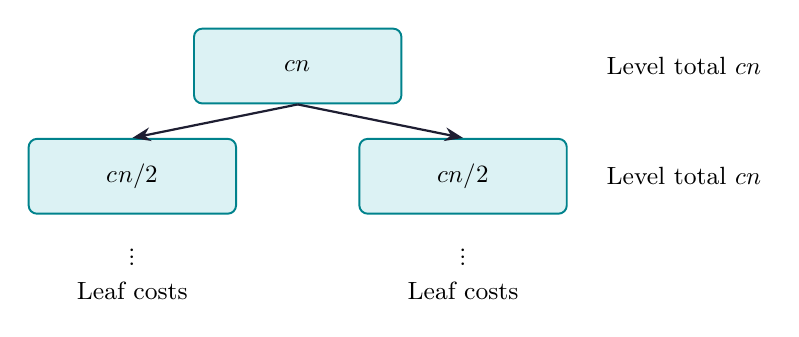
\begin{tikzpicture}[every node/.style={font=\small}]
\node[block] (root) at (0,2.1) {$cn$};
\node[block] (a) at (-2.1,0.7) {$cn/2$};
\node[block] (b) at (2.1,0.7) {$cn/2$};
\draw[arrow] (root.south) -- (a.north);
\draw[arrow] (root.south) -- (b.north);
\node[align=center] at (-2.1,-0.55) {$\vdots$\\[2pt] Leaf costs};
\node[align=center] at (2.1,-0.55) {$\vdots$\\[2pt] Leaf costs};
\node[anchor=west] at (3.8,2.1) {Level total $cn$};
\node[anchor=west] at (3.8,0.7) {Level total $cn$};
\end{tikzpicture}\par
\end{tcolorbox}

\begin{tcolorbox}[examplebox, title={A tree dominated by its leaves}]
For $T(n)=3T(n/2)+n$, level $i$ has $3^i$ subcalls of size $n/2^i$ and costs $n(3/2)^i$. If $h=\log_2 n$, there are $3^h=n^{\log_2 3}$ leaves. The internal level costs form a geometric progression with ratio $3/2$.
\[
n\sum_{i=0}^{h-1}(3/2)^i
  =2n\left((3/2)^h-1\right)
  =\Theta(n^{\log_2 3}).
\]
Including constant-cost leaves leaves the same final order.
\end{tcolorbox}

\subsection{Master theorem and its limits}
\begin{tcolorbox}[formulabox, title={Master theorem for equal subproblem sizes}]
Let $T(n)=aT(n/b)+f(n)$ with $a\ge1$, $b>1$, a constant-size base case and $p=\log_b a$. The following common forms apply.
\begin{enumerate}[leftmargin=*, itemsep=3pt, topsep=4pt]
  \item \textbf{Leaves dominate.} If $f(n)=O(n^{p-\varepsilon})$ for some $\varepsilon>0$, then $T(n)=\Theta(n^p)$.
  \item \textbf{Balanced levels.} If $f(n)=\Theta(n^p\log^k n)$ with $k\ge0$, then $T(n)=\Theta(n^p\log^{k+1}n)$. The basic exam case has $k=0$.
  \item \textbf{Root dominates.} If $f(n)=\Omega(n^{p+\varepsilon})$ and $af(n/b)\le c f(n)$ eventually for some $c<1$, then $T(n)=\Theta(f(n))$.
\end{enumerate}
\end{tcolorbox}

\par\vspace{5pt}
\begingroup
\setlength{\extrarowheight}{1pt}
\noindent\begin{tabularx}{\linewidth}{|B{4.4cm}|Y|Y|}
\hline
\textbf{Recurrence} & \textbf{Check} & \textbf{Answer} \\ \hline
$4T(n/2)+n$ & $p=2$ and $n$ is polynomially smaller than $n^2$. & $\Theta(n^2)$ \\ \hline
$2T(n/2)+n\log n$ & $p=1$, $k=1$. & $\Theta(n\log^2 n)$ \\ \hline
$2T(n/2)+n^2$ & $p=1$ and $2(n/2)^2=n^2/2$. & $\Theta(n^2)$ \\ \hline
\end{tabularx}\par
\endgroup
\begin{tcolorbox}[masonbox, title={When to choose another method}]
A recurrence with calls of sizes $n-1$, $n/3$ and $2n/3$ does not have the required equal-size pattern. For $T(n)=T(n-1)+n$, expanding yields $T(1)+\sum_{j=2}^n j=\Theta(n^2)$. For borderline functions outside the stated Master cases, use a recursion tree or prove an inductive bound directly.
\end{tcolorbox}

\newpage
\begin{center}
  {\large\bfseries\color{myred} Quick Revision --- Module 1}\\[3pt]
  {\small\color{mydark} Algorithm Analysis and Recurrence Relations $|$ ES-CS401}
\end{center}
\noindent{\color{myred}\rule{\linewidth}{1.2pt}}\par\vspace{4pt}

\begin{tcolorbox}[formulabox, title={Key Concepts at a Glance}]
\renewcommand{\arraystretch}{1.35}
\noindent\begin{tabularx}{\linewidth}{B{4.5cm}Y}
Worst-case time & $\max_{I\in\mathcal I_n} C(I)$ over all size-$n$ inputs. \\[3pt]
Average-case time & $\mathbb E[C(I)]$ under the stated input model. \\[3pt]
Triangular loop & $\sum_{i=1}^n i=n(n+1)/2$. \\[3pt]
Divide-and-conquer threshold & Compare $f(n)$ with $n^{\log_b a}$ for $aT(n/b)+f(n)$. \\[3pt]
\end{tabularx}\par
\end{tcolorbox}

\begin{tcolorbox}[defbox, title={One-Line Definitions}]
\begin{itemize}[leftmargin=*, itemsep=3pt, topsep=4pt]
  \item \textbf{Algorithm.} A finite specification of effective steps for a problem.
  \item \textbf{Loop invariant.} A property maintained across iterations.
  \item \textbf{Auxiliary space.} Peak working memory beyond the stated input and output convention.
  \item \textbf{Base case.} A small input solved directly, without further recursion.
\end{itemize}
\end{tcolorbox}

\begin{tcolorbox}[exambox, title={Frequently Asked / Viva Questions}]
\begin{enumerate}[topsep=0pt, label=\textbf{Q\arabic*.}, itemsep=5pt, leftmargin=*]
  \item \Q{What are the five standard characteristics?}
    Input, output, definiteness, finiteness and effectiveness.
  \item \Q{What establishes total correctness?}
    Partial correctness together with termination.
  \item \Q{How is a tight asymptotic bound written?}
    Use $\Theta$ after proving matching upper and lower orders.
  \item \Q{Does Big-O mean worst case?}
    Big-O is an upper bound that can be applied to any specified case function.
  \item \Q{When is linear search fastest?}
    A nonempty array whose first element matches needs one comparison.
  \item \Q{Why does average case need a distribution?}
    Each possible operation count must be weighted by its probability.
  \item \Q{What must an empirical comparison control?}
    Input size, workload family, machine, implementation settings and trial procedure.
  \item \Q{How much stack space does recursive binary search use?}
    $O(\log n)$ frames when calls are not eliminated.
  \item \Q{Why is the recursive base case essential?}
    It anchors both termination and the recurrence solution.
  \item \Q{What does the recursion tree method sum?}
    Non-recursive work at each level plus the cost of the leaves.
  \item \Q{Solve $T(n)=2T(n/2)+n$.}
    Each internal level costs $n$ and there are $\log_2 n$ levels, giving $\Theta(n\log n)$.
  \item \Q{Can the Master theorem solve a decrement-by-one recurrence?}
    Use expansion or substitution because the smaller call does not shrink by a constant factor.
\end{enumerate}
\end{tcolorbox}

\begin{tcolorbox}[tikzbox, title={Summary Comparison}]
\par\vspace{5pt}
\begingroup
\setlength{\extrarowheight}{1pt}
\noindent\begin{tabularx}{\linewidth}{|B{3.45cm}|Y|Y|}
\hline
\textbf{Method} & \textbf{Best used when} & \textbf{Check before finishing} \\ \hline
Substitution & A likely bound is available. & Check constants, base cases and the induction hypothesis. \\ \hline
Recursion tree & Level costs can be counted. & Include leaves and sum the complete series. \\ \hline
Master theorem & Calls split into equal-size subproblems. & Check the correct case and any regularity requirement. \\ \hline
\end{tabularx}\par
\endgroup
\end{tcolorbox}

\end{document}
